\documentclass{report}
\usepackage[utf8]{inputenc}
\usepackage{amsmath}
\usepackage{graphicx}

\title{Eksamensnoter - Divide and Conquer}
\author{André Oskar Andersen (wpr684)}
\date{\today}

\begin{document}
\maketitle

\section*{2.3 Designing algorithms}
\subsection*{2.3.1 The divide-and-conquer approach}
\begin{itemize}
    \item The divide-and-conquer paradigm involves three steps at each level of the recursion:
    \begin{itemize}
        \item \textbf{Divide} the problem into a number of subproblems that are smaller instances of the same problem \\
        \item \textbf{Conquer} the subproblems by solving them recursively. If the subproblem sizes are small enough, however, just solve the subroblems in a straightforward manner \\
        \item \textbf{Combine} the solutions to the subproblems into the solution for the original problem
    \end{itemize}
    \item The \textit{merge sort} algorithm closely follows the divide-and-conquer paradigm:
    \begin{itemize}
        \item \textbf{Divide:} Divide the \textit{n}-element sequence to be sorted into two subsequences of $n/2$ elements each
        \item \textbf{Conquer:} Sort the two subsequences recursively using merge sort
        \item \textbf{Combine:} Merge the two sorted subsequences to produce the sorted answer
    \end{itemize}
\end{itemize}
\subsection*{2.3.2 Analyzing divide-and-conquer algorithms}
\begin{itemize}
    \item When an algorithm contains a recursive call to itself, we can often describe its running time by a \textit{recurrence equation} or \textit{recurrence}, which describes the overall running time on a problem of size \textit{n} in terms of the running time on smaller inputs. When can then use mathematical tools to solve the recurrence and provide bounds on the performance of the algorithm
    \item We let $T(n)$ be the running time on a problem of size \textit{n}. If the problem size is small enough, say $n \leq c$ for some constant \textit{c}, the straightforward solution takes $\Theta(1)$. Suppose that our division of the problem yields \textit{a} subproblems, each of which is $1/b$ tbe size of the original. It takes time $T(n/b)$ to solve one subproblem of size $n/b$, and so it takes time $aT(n/b)$ to solve \textit{a} of them. If we take $D(n)$ time to divide the problem into subproblems and $C(n)$ time to combine the solutions to the subproblems into the solution to the original problem, we get the recurrence
    \[
        T(n) = 
        \begin{cases}
            \Theta(1) & \textit{i$n\leq c$} \\
            aT(n/b) + D(n) + C(n) & \text{otherwise}
        \end{cases}    
    \]
\end{itemize}
\subsubsection*{Analysis of merge sort}
\begin{itemize}
    \item We reason as follows to set up the recurrence for $T(n)$, the worst-case running time of merge sort on \textit{n} numbers. Merge sort on just one element takes constant time. When we have $n > 1$ elements ,we break down the running time as follows:
    \begin{itemize}
        \item \textbf{Divide:} The divide step just computes the middle of the subarray, which takes constant time. Thus, $D(n) = \Theta(1)$
        \item \textbf{Conquer:} We recursively solve two subproblems, each of size $n/2$, which contributes $2T(n/2)$ to the running time
        \item \textbf{Combine:} Merging \textit{n}-elements takes $\Theta(n)$, and so $C(n) = \Theta(n)$
    \end{itemize}
    \item Letting $D(n) + C(n) = \Theta(1) + \Theta(n) = \Theta(n)$ and adding this to the $2T(n/2)$ term from the "conquer" step gives the recurrence for the worst-case running time $T(n)$ of merge sort:
    \[
        T(n) = 
        \begin{cases}
            \Theta(1) & \text{if $n = 1$} \\
            2T(n/2) + \Theta(n) & \text{if $n > 1$}
        \end{cases}    
    \]
    \item We can use an \textit{recursion tree} to understand why $T(n) = \Theta(n \lg n)$. This is done, by first rewritting $T(n)$:
    \[
        T(n) = 
        \begin{cases}
            c & \text{if $n = 1$} \\
            2T(n/2) + cn & \text{if $n > 1$}
        \end{cases}    
    \]
    where \textit{c} represents the time requiered to solve problems of size 1 as well as the time per array element of the divide and combine steps (it is unlikely that the same constant represents both. We can get around this by letting \textit{c} be the larger/lesser of these times and understanding that our recurrence gives an upper/lower bound on the running time).
    \begin{center}
        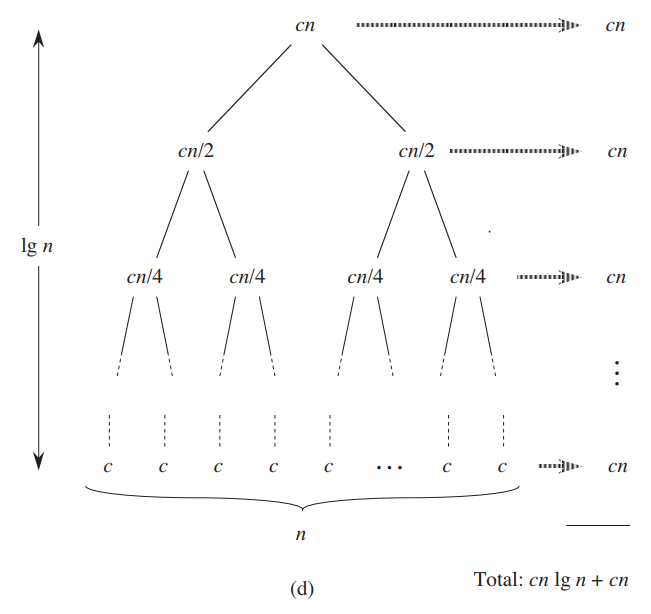
\includegraphics[width = 10 cm]{../entities/merge_sort_recursion_tree.png}
    \end{center}
    Next, we add the costs across each level of the tree. In general, the level \textit{i} below the top has $2^i$ nodes, each contributing a cost of $c(n/2^i)$, so that the \textit{i}th level below the top has total cost $2^ic(n/2^i) = cn$. \\
    The toal number of levels of the recursion tree is $\lg n + 1$, where \textit{n} is the number of leaves, corresponding to the input size. An informal inductive argument justifies this claim:
    \begin{itemize}
        \item The base case occurs when $n = 1$, in which case the tree has only one level. Since $\lg 1 = 0$, we have that $\lg n + 1$ gives the correct number of levels.
        \item Assume, that the number of levels of a recursion tree with $2^i$ leaves is $\lg 2^i + 1 = i + 1$. Because we are assuming that the input size is a power of 2, the next input size to consider is $2^{i + 1}$. A tree with $n = 2^{i + 1}$ leaves has one more level than a tree with $2^i$ leaves, and so the total number of levels is $(i + 1) + 1 = \lg 2^{i + 1} + 1$.
    \end{itemize}
    To compute the total cost represented by the recurrence $T(n)$, we add up the costs of all the levels; the tree has $\lg n + 1$ levels, each costing $cn$, for a total of $cn(\lg n + 1) = cn \lg n + cn = \Theta(n \lg n)$.
\end{itemize}

\end{document}